\section{Shared geometric and matching tools}\label{sec:frames}
The corner and frame arguments share the following geometric and matching tools.
All statements in this section are independent of the corner threshold.
Lemmas~\ref{lem:cube-incidence} and~\ref{lem:transverse-corner} state the
shape-independent facts used in the directional bounds of
Section~\ref{sec:boxes}.
The following form of Hall's theorem isolates the matching step.

\begin{lemma}[Hall criterion with a matched subset]\label{lem:partial-matching}
Consider $L$ target positions and $N\ge L$ source copies. Suppose every
source misses at most $d$ positions. If a set $P_0$ of positions can be
matched to distinct copies, and every position outside $P_0$ has at least
$d$ neighbours, then all $L$ positions can be matched.
\end{lemma}
\begin{proof}
For a position set $D\subseteq P_0$, the given matching supplies $|D|$
neighbours. If $D\nsubseteq P_0$ and $|D|\le d$, a position in
$D\setminus P_0$ alone has at least $d$ neighbours. If $|D|>d$, every
source neighbours $D$, since none can miss all its positions. In each case
Hall's inequality holds.
\end{proof}

\begin{lemma}[Missing pairs and shared corners]\label{lem:cube-incidence}
Every five-colour variety has eight distinct cyclic corner types.
An adjacent-repeat variety lacks exactly one bichromatic edge type;
an opposite-repeat variety lacks exactly two, which are disjoint.
Two disjoint missing pairs determine a unique opposite-repeat variety.
If either of two varieties is opposite-repeat, they share at least two
corner types. A target has at most one monochromatic edge; each bichromatic
type occurs on at most two edges, and a doubled type contains the repeated
colour. Thus two disjoint bichromatic types account for at most three
geometric target edges.
\end{lemma}
\begin{proof}
A missing bichromatic pair occupies opposite singleton faces: if a colour
is repeated, a face of the other colour cannot be opposite both copies.
An adjacent-repeat variety has one opposite pair of singleton faces, and an
opposite-repeat variety has two. Two disjoint missing pairs specify two
opposite face pairs, leaving the fifth colour on the remaining pair,
which determines a unique variety.

For the shared-corner assertion, let the opposite-repeat variety repeat
$r$, with singleton opposite pairs $\{\alpha,\beta\}$ and
$\{\gamma,\delta\}$. It contains both cyclic orientations of each
$rxy$ with $x\in\{\alpha,\beta\}$ and $y\in\{\gamma,\delta\}$.
In the other variety, an $r$-face with no adjacent $r$-face has at least
three distinct colours around it. Their cyclic order crosses between the
two pairs at least twice, giving two shared corners. If its $r$-faces
are adjacent, the other neighbours of each form a path of three distinct
colours. Each path crosses between the pairs and gives a shared corner,
and these have different types. Corner counts are symmetric: a five-colour
variety has eight distinct cyclic corner types, since the only repeated
colour multisets occur at the two ends of an edge, in opposite cyclic orders.

Only the repeated colour can form a monochromatic edge. Two singleton
faces meet along at most one edge; hence a doubled bichromatic type
contains the repeated colour and occurs at most twice. Two disjoint types
cannot both contain that colour, proving the final bound.
\end{proof}

\begin{lemma}[A transverse edge forces a common corner]\label{lem:transverse-corner}
Let source and target both be adjacent-repeat varieties. If the source
lacks the type of a target edge not parallel to the target's monochromatic
edge, then it shares a corner type with the target.
\end{lemma}
\begin{proof}
Relabel the colours and rotate the target to $T=(0,1,0,2,3,4)$.
Its monochromatic edge is parallel to $z$.
The types occurring on edges transverse to the monochromatic edge are
$03,04,13,14,23,24$.  The proper half-turn interchanging the $x$- and
$y$-directions and reversing $z$, followed by the colour relabelling
$1\leftrightarrow2$, $3\leftrightarrow4$, fixes $T$ and pairs these types
as $(03,04)$, $(13,24)$, and $(14,23)$.  Thus three cases suffice.
For each missing type the source has its two colours on opposite faces.
The other three colours occur around that axis in one of two cyclic
orientations.  The three adjacent-repeat choices in each orientation
share six tricoloured corners.  Reading those common corners gives:
\[
\begin{array}{c|c|c}
\text{Missing type}&\text{Shared corners in one orientation}
 &\text{Shared corners in the other orientation}\\\hline
03&024,041&123\\
13&032&041,142\\
14&013,123&024
\end{array}
\]
Every entry is nonempty, so the source and target share a corner.
\end{proof}

For a bichromatic pair $\alpha\beta$, let $\mathcal H_{\alpha\beta}$ be the family of
varieties lacking that edge type.  In every such cube, $\alpha$ and $\beta$ are
opposite singleton faces.  The four faces around this axis use the other
three colours, one of them twice.  There are nine varieties in
$\mathcal H_{\alpha\beta}$: three opposite-repeat varieties $O_r$, and six
adjacent-repeat varieties $A_r^+$ and $A_r^-$, where $r$ is the repeated
colour.  The signs distinguish the two cyclic orientations of the three
distinct ring colours.  All three $A_r^+$ varieties share the same six
tricoloured corner types; all three $A_r^-$ varieties share the reverse
six types.

\begin{lemma}[The missing-pair corner array]\label{lem:fixed-missing-pair}
The eight corners of an opposite-repeat target $O_r\in\mathcal H_{\alpha\beta}$
form a $2\times2$ array with two positions per cell. Rows correspond to
the two unordered ring-colour pairs involving $r$, and columns to their
cyclic orientations. A source $O_r$ fits every cell; the other two
opposite-repeat varieties each fit one row; and the positive and negative
adjacent-repeat varieties fit the corresponding columns.
Consequently, every variety in $\mathcal H_{\alpha\beta}$ shares at least four
corner types with every opposite-repeat variety in that family.
\end{lemma}
\begin{proof}
Each cell contains one corner at each end of the $\alpha\beta$ axis.
Reading the ring colours gives the stated incidences. Figure~\ref{fig:ring-array}
shows the example $O_2=(0,1,2,2,3,4)$ in $\mathcal H_{01}$, with $+$
chosen to include $023$. Relabelling the three ring colours gives the
other two targets, and relabelling the palette gives every missing-pair
family. Cyclic rotations identify corner labels. In particular, the
two positions in each cell have identical source neighbourhoods.
\end{proof}

\begin{figure}[ht]
\centering
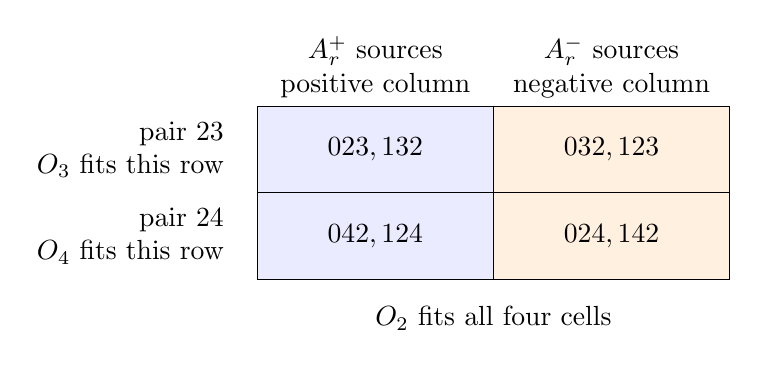
\begin{tikzpicture}[x=3cm,y=1.1cm]
\fill[blue!8] (0,0) rectangle (1,2);
\fill[orange!12] (1,0) rectangle (2,2);
\draw (0,0) rectangle (2,2);
\draw (1,0)--(1,2); \draw (0,1)--(2,1);
\node at (.5,1.5) {$023,132$};
\node at (1.5,1.5) {$032,123$};
\node at (.5,.5) {$042,124$};
\node at (1.5,.5) {$024,142$};
\node[align=center] at (.5,2.45) {$A_r^+$ sources\\positive column};
\node[align=center] at (1.5,2.45) {$A_r^-$ sources\\negative column};
\node[anchor=east,align=right] at (-.1,1.5) {pair $23$\\$O_3$ fits this row};
\node[anchor=east,align=right] at (-.1,.5) {pair $24$\\$O_4$ fits this row};
\node at (1,-.45) {$O_2$ fits all four cells};
\end{tikzpicture}
\caption{Corner array of $O_2$ in the family lacking $01$.
Each cell contains two target positions. Here $r\in\{2,3,4\}$;
all three adjacent-repeat sources of a given sign fit the same column.}
\label{fig:ring-array}
\end{figure}

\subsection{Signed corner projections}
Retain the family $\mathcal H_{\alpha\beta}$ from Lemma~\ref{lem:fixed-missing-pair},
with its opposite-repeat varieties and their $2\times2$ corner array.
Write $C(W)$ for the cyclic corner types of $W$.

\begin{lemma}[Corner projections onto a missing-pair family]\label{lem:thin-projections}
Fix a bichromatic pair $\alpha\beta$.  Let $C^+$ and $C^-$ be the two sets of six
tricoloured corner types shared by the three adjacent-repeat varieties of
the respective cyclic orientations in $\mathcal H_{\alpha\beta}$.  An
opposite-repeat variety in $\mathcal H_{\alpha\beta}$ has four corners in each set.
For a source $W\notin\mathcal H_{\alpha\beta}$, put
\[
 p(W)=|C(W)\cap C^+|,\qquad m(W)=|C(W)\cap C^-|.
\]
Then
\[
 (p(W),m(W))\in\{(4,0),(2,1),(1,2),(2,2),(0,4)\}.
\]
\end{lemma}

\begin{proof}
Relabel the poles as $0,1$ and the ring colours as $2,3,4$.  Choose the
positive orientation so that
\[
 C^+=\{023,034,042,124,132,143\},\qquad
 C^-=\{024,032,043,123,134,142\}.
\]
Triples denote cyclic classes; face order is $(+x,-x,+y,-y,+z,-z)$.  The following table gives representatives of
all geometric cases outside $\mathcal H_{01}$, up to a colour permutation
preserving the pole pair and a simultaneous reflection, which may exchange
$C^+$ and $C^-$.  Such a reflection is only a symmetry of this incidence
calculation, not an allowed assembly move.
\[
\begin{array}{c|cc}
 W&p(W)&m(W)\\\hline
 (0,0,1,2,3,4)&2&2\\
 (0,1,0,2,3,4)&0&4\\
 (0,2,0,3,1,4)&2&1\\
 (0,2,1,2,3,4)&0&4\\
 (0,2,1,3,2,4)&2&1\\
 (0,2,1,3,4,4)&2&2
\end{array}
\]
To see that these cases exhaust the possibilities, first suppose a pole
colour is repeated.  Its two faces are either opposite, or adjacent; in
the latter case the other pole is opposite one repeated face or adjacent
to both.  If a ring colour is repeated, the two pole faces must be
adjacent, since otherwise $W$ belongs to $\mathcal H_{01}$.  Fix them at
$x^+$ and $y^+$.  Among the remaining faces $x^-,y^-,z^+,z^-$, an opposite
repeated pair is $z^+,z^-$.  An adjacent repeated pair is either $x^-,y^-$,
or one of $x^-,y^-$ together with one of $z^+,z^-$.  These are the final
three rows.

Each entry follows by reading the eight corners of the displayed cube.
The projections of the nine family
varieties themselves are $(6,0),(0,6)$, and $(4,4)$, as follows directly
from their ring descriptions.
\end{proof}

\begin{lemma}[Compatibility for a thin frame]\label{lem:thin-compatibility}
Choose an orientation of a five-colour target for a $2\times2\times3$
frame such that its four noncorner edge positions are bichromatic.
Every source cube fits at least four of the twelve positions.
\end{lemma}

\begin{proof}
If either source or target is opposite-repeat,
Lemma~\ref{lem:cube-incidence} gives two shared corners.
The four parallel bichromatic edges have either four distinct types or
two types occurring twice each. In the latter case both contain the
target's repeated colour. The source's missing pairs are disjoint, so
it fits at least two of these edges, giving four compatible positions.

If both varieties are adjacent-repeat, the four parallel edge types are
distinct and transverse to the monochromatic edge. The source fits either
all four, or at least three and a corner by
Lemma~\ref{lem:transverse-corner}. Again it fits four positions.
\end{proof}

\subsection{Eight family cubes and three arbitrary additions}

% Analytic lemma for the 2 x 2 x 3 five-colour problem.

\begin{lemma}[Eight cubes with a common missing pair]\label{lem:eight-common-missing}
Eight cubes from $\mathcal H_{\alpha\beta}$, together with any three additional
five-colour cubes, have a corner solution whose target belongs to
$\mathcal H_{\alpha\beta}$.
\end{lemma}

\begin{proof}
Let $O,P,Q$ count the opposite-repeat, positive
adjacent-repeat, and negative adjacent-repeat copies among the chosen eight.
Thus $O+P+Q=8$; $C^+$ and $C^-$ are as in Lemma~\ref{lem:thin-projections}.

If $O+\min(P,Q)\ge4$, the $2\times2$ Hall argument gives an
opposite-repeat corner solution from these eight copies alone. Explicitly,
choose $O_r$ whose opposite-repeat multiplicity is maximal. Each cell has
at least $O/2+\min(P,Q)\ge2$ neighbours, each row has at least
$8-O/2\ge4$, and each column has at least $O+\min(P,Q)\ge4$.
Every other nonempty union of cells has all eight copies as neighbours.

Otherwise exchange the signs so that $O+Q\le3$. Put
$\kappa=O+Q=8-P$, so $P\ge5$ and $0\le \kappa\le3$.
Some positive variety $A_r^+$ occurs at least twice. If its eight
corners have a matching among all eleven copies, we are done. Otherwise,
choose a deficient Hall set $D$ of its corners. The two copies of
$A_r^+$ fit every corner, so $|D|\ge3$ and $D$ contains a tricoloured
corner. All $P$ positive copies are therefore neighbours of $D$.
Let $R$ be its other neighbours and put $U=C^+\setminus D$, $u=|U|$.
Since $|D|+u\le8$,
\[
 P+|R|<|D|\le8-u,\qquad |R|+u\le \kappa-1.
\]
Remove the $P$ positive copies and the copies in $R$. Every surviving
copy has all its positive corners in $U$, and $u\le2$.

Every family opposite-repeat variety has four corners in $C^+$, so no
such chosen copy remains. At least
\[
 \kappa-|R|\ge u+1
\]
of the chosen nonpositive copies remain, and all of them are negative
adjacent-repeat copies. Each fits every corner in $C^-$. The remaining
pool has at least
\[
 \kappa+3-|R|\ge4+u
\]
copies.

Lemma~\ref{lem:thin-projections} gives the following implications for every source:
\[
\begin{array}{c|ccc}
 |C(W)\cap C^+|\le u &u=0&u=1&u=2\\\hline
 |C(W)\cap C^-|\ge&4&2&1.
\end{array}
\]
Indeed, the family varieties have projection sizes $(6,0),(0,6),(4,4)$,
and every variety outside the family has one of
$(4,0),(2,1),(1,2),(2,2),(0,4)$.

Partition $C^-$ into three pairs, indexed by the unordered pairs of ring
colours. The negative half of each family opposite-repeat target is the
union of two of these pairs. We will match one such four-position half
using the remaining pool, then use four positive copies for its positive
half.

Let $j$ be the number of negative-family copies in the remaining pool;
thus $j\ge u+1$. If $j\ge4$, the conclusion is immediate. If $j=3$,
another remaining copy fits at least one negative corner; choose a target
whose negative half contains it and fill the other three positions with
negative-family copies.

If $j=2$, then $u\le1$. Two other remaining copies each fit at least two
negative corners, so they can be assigned distinct ones. Any two negative
corners lie in the union of two of the three pairs. Choose the corresponding
opposite-repeat target and fill its other two negative positions with the
two negative-family copies.

Finally, if $j=1$, then $u=0$, and there are at least three other copies,
each fitting at least four of the six negative corners. Choose one of
these copies $W$. Some union of two of the three pairs contains at least
three of its negative corners. In that four-position half, every other
copy fits at least two positions. Hence $W$ and any two other copies can
be matched to three distinct positions: two copies have at least two
neighbours, and all three together have at least three. The one
negative-family copy fills the fourth position.

In every case we obtain the negative half of an opposite-repeat target
in $\mathcal H_{\alpha\beta}$. Four of the $P\ge5$ positive copies fill its
positive half. The positive copies used here are disjoint from the surviving pool. This proves the lemma.
\end{proof}


